\section{Spin Orbit Coupling}

When zooming in on the oscillations of the longitudinal resistivity, 
a beating pattern is visible.
This behaviour increases for high $U_\text{gate}$.
The resistivity for $U_\text{gate} = 1.5V$ and $1.4K$ is depicted in fig. \ref{fig:beatingPattern}.
This behaviour is likely caused by the Rashba effect, which is based on spin orbit coupling.
\begin{figure}[h]
    \centering
    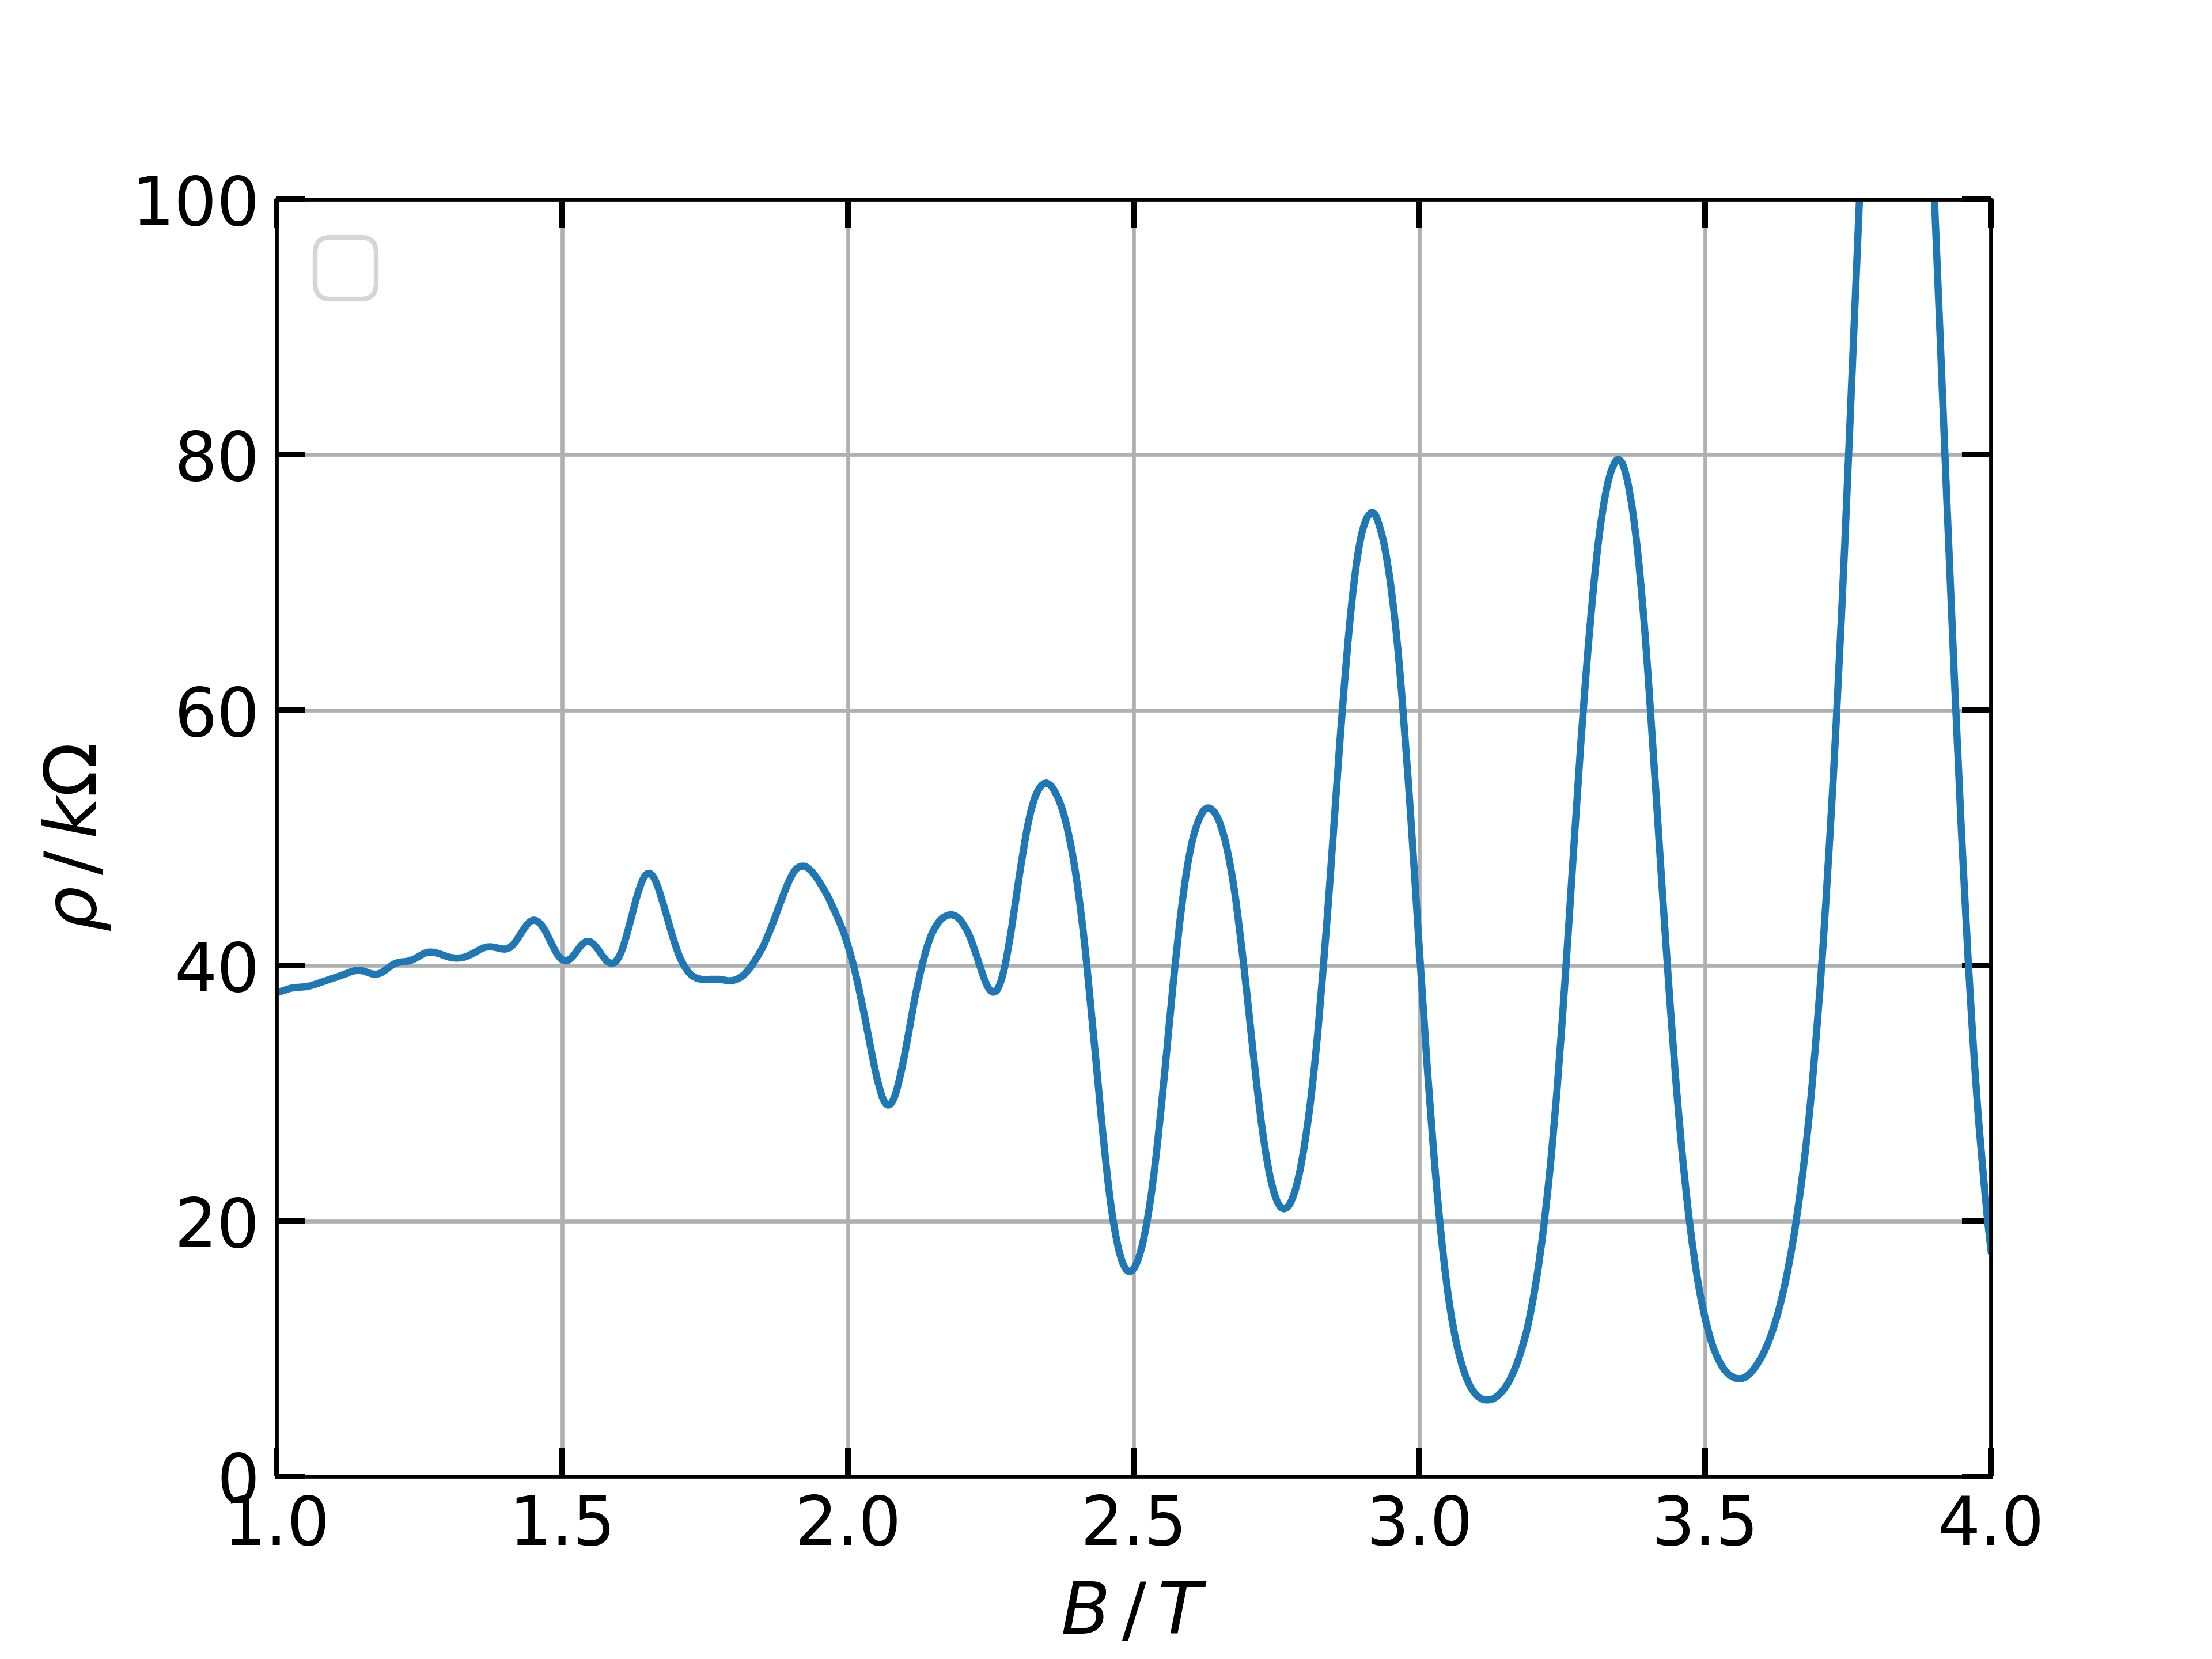
\includegraphics[width=0.45\textwidth]{../Images/beatingPattern.png}
    \caption{Longitudinal resistivity $\rho_\text{xx}$ for high $U_\text{gate} = 1.5V$ at $1.4K$.
    A beating pattern is visible.
    }
    \label{fig:beatingPattern}
\end{figure}
